\thispagestyle{plain}

\noindent In the first part of this project a function called Franke function was used as the data analysed. The Franke function is given by the following equation:
\begin{align*}
    f(x,y) &= \frac{3}{4} \, exp\left(- \frac{(9x-2)^2}{4} - \frac{(9y-2)^2}{4}\right) \\
    &+ \frac{3}{4}\, exp\left( - \frac{(9x +1)^2}{49} - \frac{(9y+1)}{10}\right) \\
    &+ \frac{1}{2}\, exp\left( -\frac{(9x-7)^2}{4} - \frac{(9y-3)^2}{4}\right) \\
    &- \frac{1}{5} exp \left( - (9x -4)^2 - (9y-7)^2\right)
\end{align*}
A graphic representation is shown in figure \eqref{Franke function}
\begin{figure}[H]
	\centering
	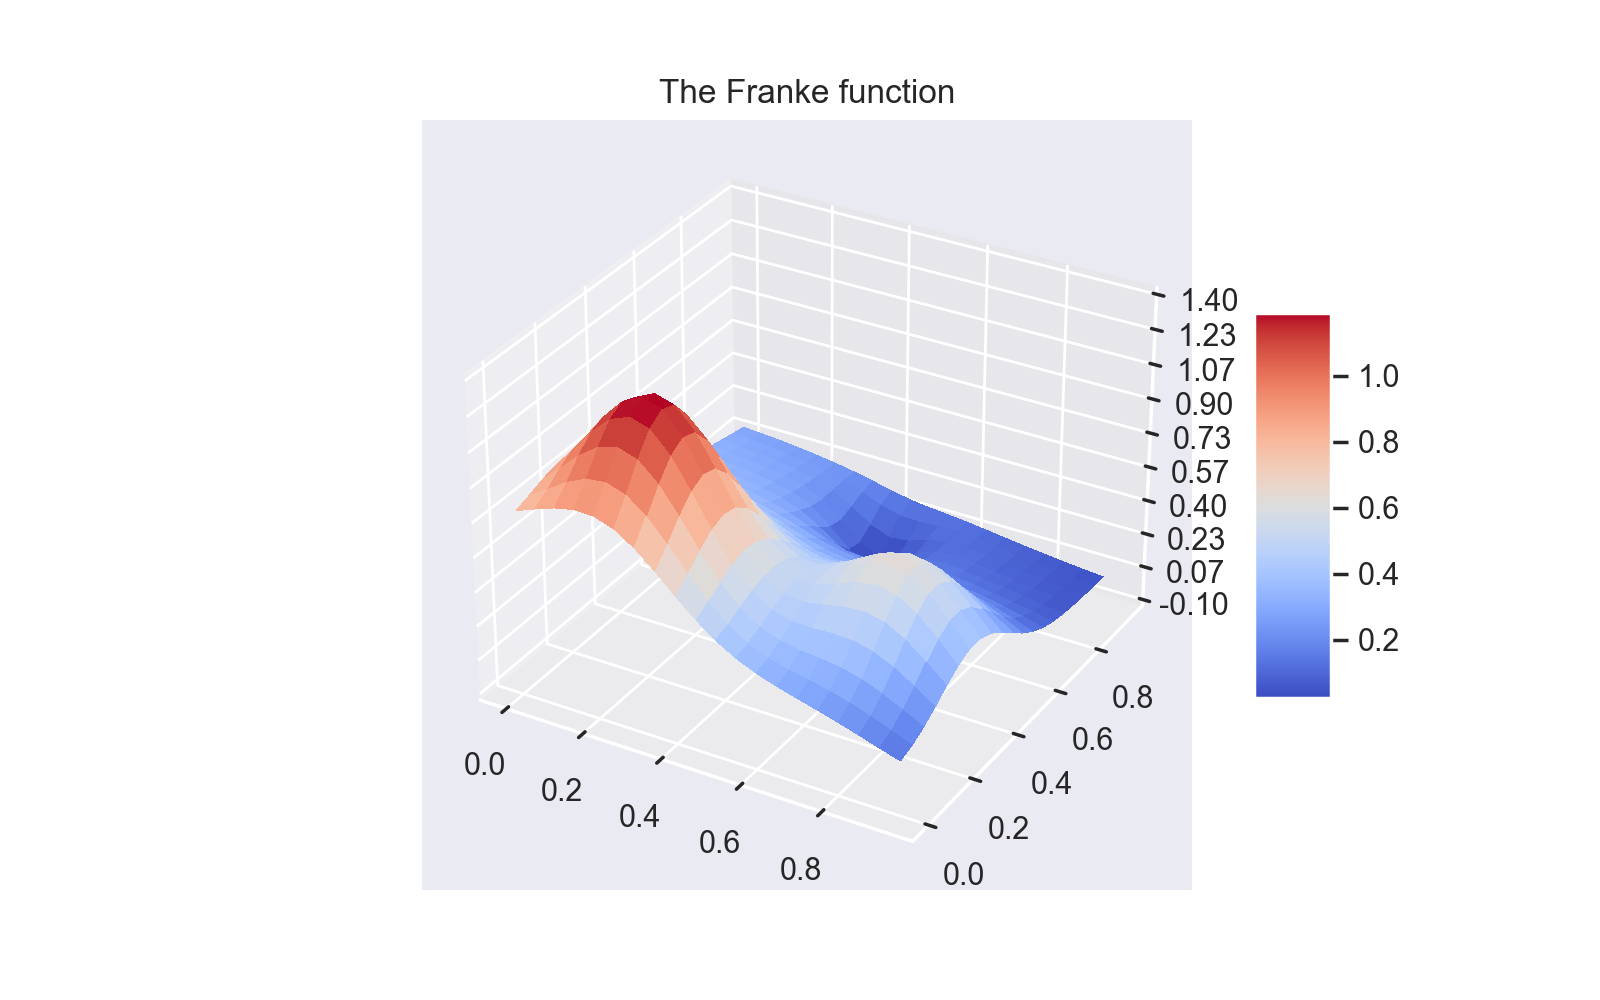
\includegraphics[width=0.5\textwidth]{Figure_1.png}
	\caption{\centering A plot of the Franke function }
	\label{Franke function}
\end{figure}
\noindent This function was fitted with the OLS method, were a polynomial with degree 5 was used to create the design matrix. Since the design matrix in this case was noninvertible, singular value decomposition was used to create the $\beta$-values needed to create a model of the dataset. The mean square error and the R2 score was calculated for both the testing and training datasets. \newline \newline

\noindent Next Ridge regression was used on the Franke function, to see if this method have a better fit than what was obtained with OLS. Diffrent values for $\lambda$ was used to obtain the best fit as possible.
